\newpage
\section{Experiments Analysis}
In order to extract data out of the simulator, several experiments were run using various settings. A set of base parameters were determined for each experiment. These parameters are then adjusted to dependent on the scenario.
The base case was determined to be:
\begin{itemize}
    \item Inflow [vehicle/min] = 35 \cite{Green2020GuideTT}
    \item Simulation Time [min] = 20
    \item Average driver mood = 0.85
    \item Number of lanes = 4
    \item Highway length [km] = 10
    \item Speed limit [km/h] = 110
    \item Proportion of Autonomous cars = variable
    \item Proportion of Trucks = 0.0 % 10% normal
\end{itemize}
For all experiments, the proportion of autonomous cars were varied, to extract results 0.0 to 1.0 in 0.1 intervals. Additionally, for each of the experiments, one of the following parameters was varied based on a predetermined range. The experiment was run with varying inflow, number of lanes, speed limit, and proportion of trucks. This was done to account for the randomness factor of the simulations, since a favourable or unfavourable random seed could lead to skewed results. Furthermore, to account for the randomness factor, the simulation was run 20 times, and the average of these results was calculated. 
The experiments were run without any of the visualization described in the previous section, as it was not needed for them. Finally, for each simulation the amount of cars passing the highway (referred to as traffic flow) and the average speed of the cars were recorded. The higher the flow rate \& average speed the better. 

Running 20 simulations for each combination of two variable data points means that each experiment consist of 1200 to 2000 simulations. To speed things up, they are run concurrently using multi-threading. Even with multi-threading it took more than six hours to run all these simulations on the machine used. Some simulations, especially the ones with greater inflow and greater number of cars, require more computational time than others as multiple loops involving vehicle instances are running in the simulation.

\subsection{Experiments with varying inflow}
The experiments were done with varying inflow to show the effect different proportions of autonomous cars has on the traffic inflow. This will also show if there are specific levels of inflow, where autonomous cars have a bigger or smaller impact on the traffic flow. The inflow is varied from 10 to 60 at steps of 10. Along with the 11 different values for proportion of autonomous cars, it gives a total of 66 data points, each consisting of 20 simulations.
As we are focusing on the autonomous cars, the proportion of trucks is 0 in this experiment.

\begin{figure}[H]
    \centering
    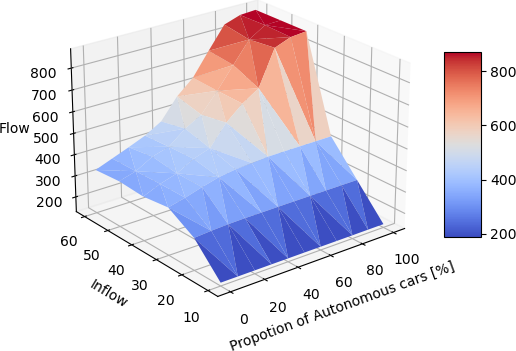
\includegraphics[width=0.5\textwidth]{images/Experiment1.png}
    \caption{Experiments with varying inflow}
    \label{fig:experiment1}
\end{figure}

The results of this experiment, which can be seen in figure \ref{fig:experiment1},  shows that at low inflow (<30), the amount of autonomous cars does not have any significant change the traffic flow. However, on higher inflow there is a close to linear correlation, where more autonomous cars means higher traffic flow. At inflow > 30, the traffic flow is more than doubled between 0\% and 100\% autonomous cars. 
\begin{figure}[H]
    \centering
    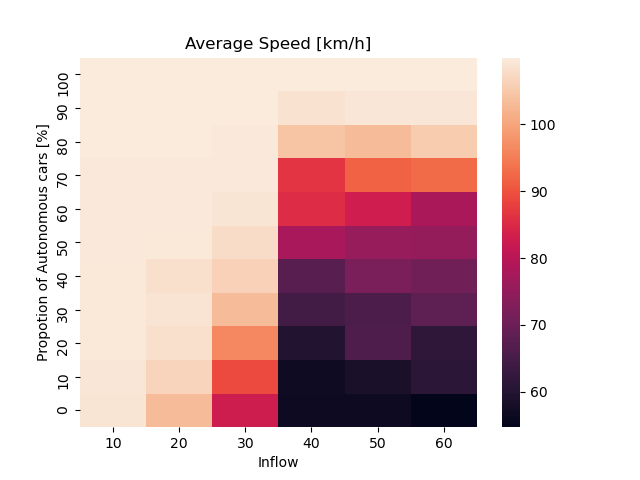
\includegraphics[width=\linewidth]{images/Experiment1-Speed.png}
    \caption{Heatmap for experiments with varying inflow}
    \label{fig:experiment1heatmap}
\end{figure}
A heatmap visualizing the average speed can be seen in figure \ref{fig:experiment1heatmap}. When looking at the average speed, the speed limit is reach fairly easily for inflow $\leq 30$, while for inflow > 30 more than 80\% autonomous cars are needed to reach the speed limit. This corresponds to the above results for traffic flow.

\subsection{Experiments with varying number of lanes}
The purpose of this experiment was to determine whether the autonomous cars needed a minimum number of lanes before they were effective, and to determine if too many lanes negates the effect of autonomous cars. The number of lanes was varied from 1 to 9 lanes, which along with the varied proportion of autonomous cars gives a total of 99 data points each consisting of 20 simulations. As we are focusing on the autonomous cars, the proportion of trucks is 0 in this experiment. 

\begin{figure}[H]
    \centering
    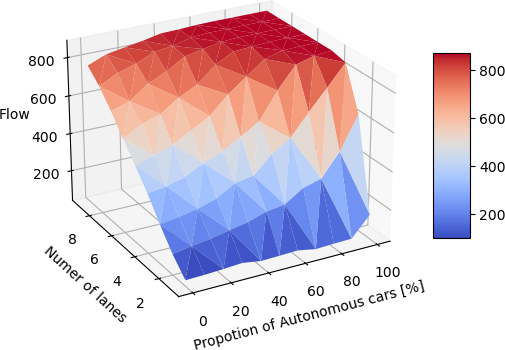
\includegraphics[width=0.5\textwidth]{images/Experiment2.png}
    \caption{Experiments with varying number of lanes}
    \label{fig:experiment2}
\end{figure}

The results of this experiment, which can be seen in figure \ref{fig:experiment2}, shows that the traffic flow hits a maximum when number of lanes, and proportion of autonomous cars increase. With 4 lanes the maximum is hit at around 80\% autonomous cars, and with more lanes  fewer autonomous cars are needed needed to  reach the max. It also shows that for autonomous cars to have any impact on the traffic  flow, at least two lanes are needed, but preferably three or more.

Similar results can also be seen when looking at the data for average speed, where a clear diagonal line is formed, indicating that more lanes and more autonomous cars are equally effective at increasing the average speed. This can be seen visualized in a heatmap in figure \ref{fig:experiment2heatmap}. 
\begin{figure}[H]
    \centering
    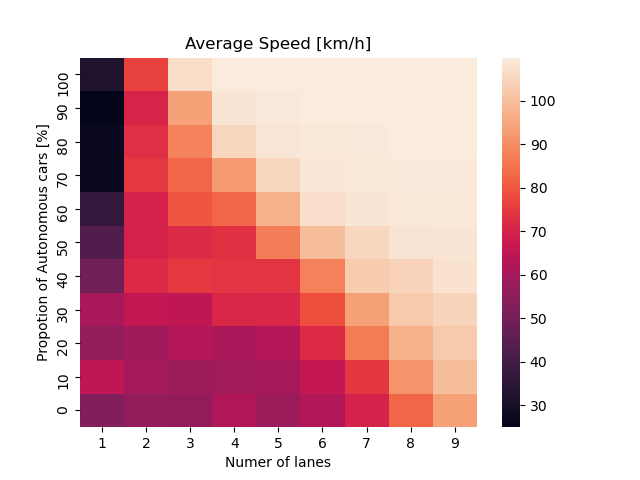
\includegraphics[width=\linewidth]{images/Experiment2-Speed.png}
    \caption{Heatmap for experiments with varying number of lanes}
    \label{fig:experiment2heatmap}
\end{figure}


\subsection{Experiments with varying speed limit}
This experiment was done to determine if changing the speed limit has an effect on the impact of autonomous cars. The speed limit is varied from 50 to 130 at 10 step intervals, along with the varied proportion of autonomous cars, it gives a total of 99 data points of 20 simulations each.  As we are focusing on the autonomous cars, the proportion of trucks is 0 in this experiment.
\begin{figure}[H]
    \centering
    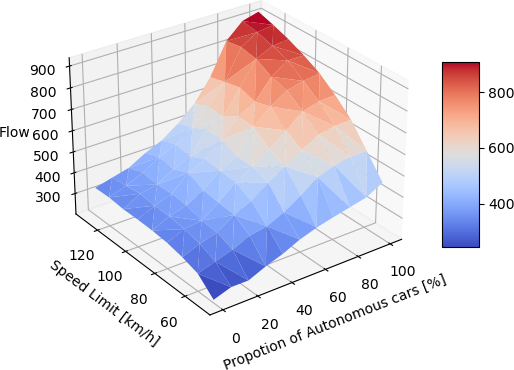
\includegraphics[width=0.5\textwidth]{images/Experiment3.png}
    \caption{Experiments with varying speed limit}
    \label{fig:experiment3}
\end{figure}
In figure \ref{fig:experiment3} the results of this experiment can be seen. This indicates that a higher speed limit increases the impact of more autonomous cars. The curve for the results with 0.0 autonomous cars quickly hits a plateau, while it gets steeper the more autonomous cars are added. 

Looking at the average speed, the results again show that more than 80\% autonomous cars, makes the average speed close the the speed limit. This is visualized as a heatmap in figure \ref{fig:experiment3heatmap}. 
\begin{figure}[H]
    \centering
    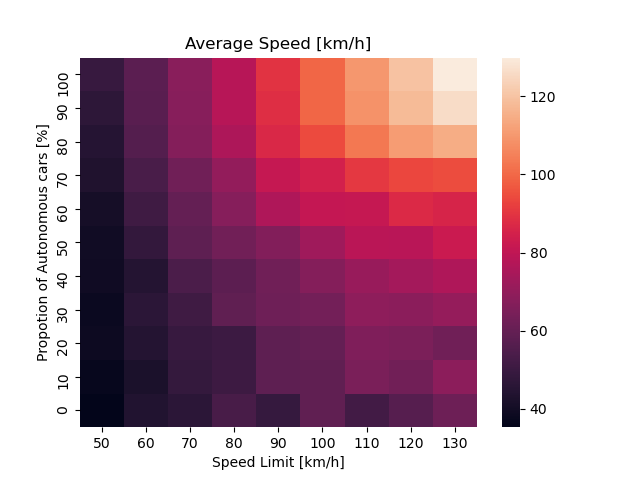
\includegraphics[width=\linewidth]{images/Experiment3-Speed.png}
    \caption{Heatmap for experiments with varying speed limit}
    \label{fig:experiment3heatmap}
\end{figure}
Both results also show that at at least 40\%-50\% autonomous cars are needed before increasing the speed limit will make any significant change to the traffic flow and average speed. This will primarily be due to this phantom traffic preventing the higher speed limit to be fully utilized.


\subsection{Experiments with varying amount of trucks}
The final experiment was done to determine what effect slow vehicles like trucks have on the impact of autonomous. This experiment limited the variables to where the sum of the two variables was less than or equal to 1. This was done because they are represented as percent of the total cars, so if the sum is more than 1, then there are more than 100\% cars.

\begin{figure}[H]
    \centering
    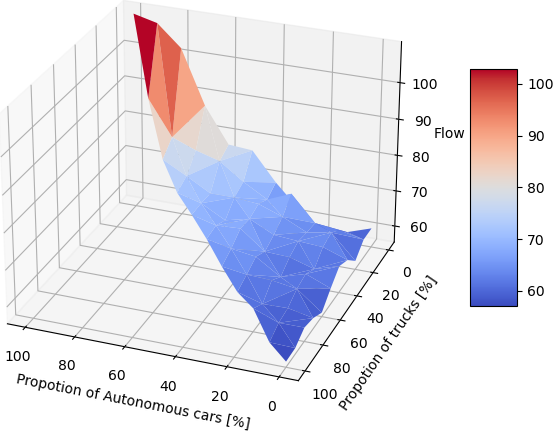
\includegraphics[width=0.5\textwidth]{images/Experiment4.png}
    \caption{Experiments with varying proportion of trucks}
    \label{fig:experiment4}
\end{figure}

The results of this experiment still shows that more autonomous cars mean higher traffic flow. It again shows the best results with more than 80\& autonomous cars, however in this case, the overall traffic flow is much lower than the other experiments, at all proportions of trucks.

%\subsection{Base experiment with no Autonomous cars}
%\subsection{Experiments with different number of Autonomous cars}
%\subsection{Experiment with only Autonomous cars}